%%% LaTeX Template: Article/Thesis/etc. with colored headings and special fonts
%%%
%%% Source: http://www.howtotex.com/
%%% Feel free to distribute this template, but please keep to referal to http://www.howtotex.com/ here.
%%% February 2011
%%%
%%% Modified May 2018 by CDM

%%%  Preamble
\documentclass[11pt,letterpaper]{article}
\usepackage[margin=1.0in]{geometry}
\usepackage[T1]{fontenc}
\usepackage[bitstream-charter]{mathdesign}
\usepackage[latin1]{inputenc}					
\usepackage{amsmath}						
\usepackage{xcolor}
\usepackage{cite}
\usepackage{hyphenat}
\usepackage{graphicx}
\usepackage{float}
\usepackage{subfigure}
\usepackage{sectsty}
\usepackage[compact]{titlesec} 
\usepackage[tablegrid]{vhistory}
\allsectionsfont{\color{accentcolor}\scshape\selectfont}

%%% Definitions
\definecolor{accentcolor}{rgb}{0.3,0.0,0.3} 
\newcommand{\teamname}{Team 5 -- Jovial McNulty}
\newcommand{\productname}{JEN - UR5 Jenga-playing Robot Arm}
\newcommand{\coursename}{CSE 4316: Senior Design I}
\newcommand{\semester}{Fall 2018}
\newcommand{\docname}{System Requirements Specification}
\newcommand{\department}{Department of Computer Science \& Engineering}
\newcommand{\university}{The University of Texas at Arlington}
\newcommand{\authors}{Joe Cloud \\ Gabriel Comer \\ Carlos Crane \\ Sammy Hamwi \\ Maxwell Sanders}

%%% Headers and footers
\usepackage{fancyhdr}
	\pagestyle{fancy}						% Enabling the custom headers/footers
\usepackage{lastpage}	
	% Header (empty)
	\lhead{}
	\chead{}
	\rhead{}
	% Footer
	\lfoot{\footnotesize \teamname \ - \semester}
	\cfoot{}
	\rfoot{\footnotesize page \thepage\ of \pageref{LastPage}}	% "Page 1 of 2"
	\renewcommand{\headrulewidth}{0.0pt}
	\renewcommand{\footrulewidth}{0.4pt}

%%% Change the abstract environment
\usepackage[runin]{abstract}			% runin option for a run-in title
%\setlength\absleftindent{30pt}			% left margin
%\setlength\absrightindent{30pt}		% right margin
\abslabeldelim{\quad}	
\setlength{\abstitleskip}{-10pt}
\renewcommand{\abstractname}{}
\renewcommand{\abstracttextfont}{\color{accentcolor} \small \slshape}	% slanted text

%%% Start of the document
\begin{document}

%%% Cover sheet
{\centering \huge \color{accentcolor} \sc \textbf{\department \\ \university} \par}
\vspace{1 in}
{\centering \huge \color{accentcolor} \sc \textbf{\docname \\ \coursename \\ \semester} \par}
\vspace{0.5 in}
\begin{figure}[h!]
	\centering
   	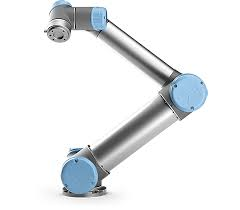
\includegraphics[width=0.45\textwidth]{images/ur5}
\end{figure}
\vspace{0.5 in}
{\centering \huge \color{accentcolor} \sc \textbf{\teamname \\ \productname} \par}
\vspace{0.5 in}
{\centering \large \sc \textbf{\authors} \par}
\newpage


%\vspace{1 in}
%\centerline{January 13th, 2012}
%\newpage

%%% Revision History
\begin{versionhistory}
  	\vhEntry{0.1}{10.19.2018}{SH}{document creation}
  	\vhEntry{0.2}{10.05.2015}{JC|GC|CC|SH|MS}{complete draft}
\end{versionhistory}
\newpage

%%% Table of contents
\setcounter{tocdepth}{3}
\tableofcontents
\newpage

%%% List of figures and tables (optional)
\listoffigures
%\listoftables
\newpage

\section{Product Concept}
The objective of this project is to implement a Jenga-playing robot system involving a human opponent. Our solution will utilize 3D computer vision to develop scans of the tower's state, and a vacuum gripper to grip blocks. The human opponent will take turns with the robot performing block pulls and placing them at the top of the stack. The goal isn't necessarily to defeat the human opponent, but build a system capable of make multiple moves prior to the tower collapsing. 

\subsection{Purpose and Use}
This project serves as an interactive demonstration of computer science concepts with the goal of inspiring the next generation of scientists \& engineers. This product is designed to engage K-12 students at showcases and university outreach events. Students are expected to engage with the product by taking turns with the robot in a fun, friendly game of Jenga.

\subsection{Intended Audience}
This product is intended to be used by the university, College of Engineering, or the Computer Science \& Engineering Department as a recruiting tool for future engineering students. Making this product available commercially to other universities and companies is possible. Though, as this is an end-to-end system designed to demonstrate the possibilities as a STEM student at UT Arlington, it is intended to be administered on behalf of the university. The end-user of this system is a member of the general public. Mattel$\circledR$ states that Jenga is appropriate for players ages six and up.

\begin{figure}[h!]
	\centering
   	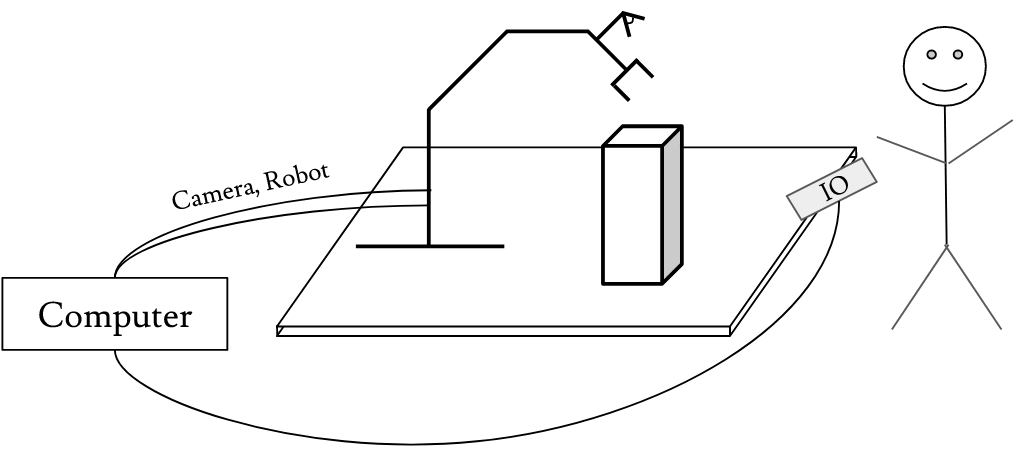
\includegraphics[width=0.90\textwidth]{images/system_setup}
    \caption{System concept drawing}
\end{figure}

\newpage
\section{Product Description}
This section provides the reader with an overview of The UR5 Jenga Playing Robot. The primary operational aspects of the product, from the perspective of the end users and maintainers, are defined here. The primary features and functions found in the product, as well as user interfaces are described in this section. Reference Figure 1 for a conceptual drawing of the product. 


\subsection{Features \& Functions}
The UR5 Jenga Playing Robot will have the following features \& functions, referencing Figure 1:
\begin{itemize}
    \item Robotic arm for movement and 3D scanning, a Universal Robotics 5 robotic arm
    \item Camera, a 3D camera array
    \item Computer package, likely an Intel NUC
    \item Gripping component
    \item IO device, a physical button with wires connecting it to the computer package
\end{itemize}

\subsection{External Inputs \& Outputs}
The only external data flow used in The UR5 Jenga Playing Robot will be the single IO device pressed by the user to inform the system that their turn is complete.

\subsection{Product Interfaces}
There will be no graphical user interface for this product. See Figure 1 for a mock-up of the physical user IO device interface that will be used. 
\newpage
\section{Customer Requirements}
%Include a header paragraph specific to your product here. Customer requirements are those required features and functions specified for and by the intended audience for this product. This section establishes, clearly and concisely, the "look and feel" of the product, what each potential end-user should expect the product do and/or not do. Each requirement specified in this section is associated with a specific customer need that will be satisfied. In general Customer Requirements are the directly observable features and functions of the product that will be encountered by its users. Requirements specified in this section are created with, and must not be changed without, specific agreement of the intended customer/user/sponsor.
This section covers the features and functions that can be expected from the UR5 Jenga-Playing Robot. Every requirement in this section is associated with a specific customer need that we need to satisfy. Our customers include: ourselves, our sponsor, our class, and the college of engineering. The features covered in this section are directly observable and should be transparent to the customer who expects the requirement. Any of the requirements below should not be changed without the agreement of the affected customer.

\subsection{Input Interface}
\subsubsection{Description}
The user interface of the UR5 will be simple and intuitive. It shall be a button that determines when the player move is completed, and the robot move is ready to begin. 
\subsubsection{Source}
Maxwell
\subsubsection{Constraints}
The button should not take up a considerable amount of space, and should not interfere with the game. Pressing the button should not shake the tower.
\subsubsection{Standards}
N/A
\subsubsection{Priority}
High

\subsection{Output Interface}
\subsubsection{Description}
The output interface will be a LED that indicates whether or not the robot has completed its turn.
\subsubsection{Source}
Maxwell
\subsubsection{Constraints}
The LED will not be blinding, and should not interfere with the vision system of the robot as well as the vision of the player. The LED should not affect the gameplay.
\subsubsection{Standards}
N/A
\subsubsection{Priority}
Low

%Added by Gabe
\subsection{Custom Jenga Tower}
\subsubsection{Description}
The UR5 Jenga-Playing Robot shall include with it for use in demonstrations, one custom Jenga tower. The tower shall be comprised of 54 3D printed blocks, each block. 
\subsubsection{Source}
Gabriel Comer
\subsubsection{Constraints}
3D printing takes a lot of time, so having to print a new tower if our first attempt is too small, too heavy, or has too much static friction, could add significant delays. Also, printing 54-block towers could become costly as we try different block types and iterate through block size and material options.
\subsubsection{Standards}
N/A
\subsubsection{Priority}
Medium

\subsection{Turn Autonomy}
\subsubsection{Description}
The UR5 Jenga-Playing Robot shall pull blocks from the tower and place them on the top without intervention by the user. Once the users has signalled the end of their turn through the button, the user will not be required to touch the tower, or interact with the display in any way, until their next turn. User intervention might improve the UR5 Jenga-Playing Robot's performance, but it would also decrease the excitement of the game being played.
\subsubsection{Source}
Gabriel Comer%it says we can use 'specified team member by name', so I just put my name
\subsubsection{Constraints}
Lack of user intervention will likely decrease the block pulling success rate of the UR5 Jenga-Playing Robot. In cases where the tower is crooked, or leaning to one side, the UR5 Jenga-Playing Robot may have difficulty obtaining accurate scans of the tower, and pulling blocks without knocking the tower down.
\subsubsection{Standards}
N/A
\subsubsection{Priority}
High


%\subsubsection{Description}
%Detailed requirement description...
%\subsubsection{Source}
%Source
%\subsubsection{Constraints}
%Detailed description of applicable constraints...
%\subsubsection{Standards}
%List of applicable standards
%\subsubsection{Priority}
%Priority

%\subsection{Requirement Name}
%\subsubsection{Description}
%A detailed description of the feature/function that satisfies the requirement. For example: \textit{The GUI background will be slate blue. This specific color is required in order to ensure that the GUI matches other similar software products offered by the customer. Slate blue is specified as \#007FFF, using six-digit hexadecimal color specification.} It is acceptable and advisable to include drawings/graphics in the description if it aids understanding of the requirement.
%\subsubsection{Source}
%The source of the requirement (e.g. customer, sponsor, specified team member (by name), federal regulation, local laws, CSE Senior Design project specifications, etc.)
%\subsubsection{Constraints}
%A detailed description of realistic constraints relevant to this requirement. Economic, environmental, social, political, ethical, health \& safety, manufacturability, and sustainability should be discussed as appropriate.
%\subsubsection{Standards}
%A detailed description of any specific standards that apply to this requirement (e.g. \textit{NSTM standard xx.xxx.x. color specifications \cite{Rubin2012}}. Standards exist for practically everything (ATC standard fuses, IEEE 802.15.4 embedded wireless, TLS 1.3 encryption, etc.), so be sure that you research and document which ones will be followed in meeting this requirement.
%\subsubsection{Priority}
%The priority of this requirement relative to other specified requirements. Use the following priorities:
%\begin{itemize}
%\item Critical (must have or product is a failure)
%\item High (very important to customer acceptance, desirability)
%\item Moderate (should have for proper product functionality);
%\item Low (nice to have, will include if time/resource permits)
%\item Future (not feasible in this version of the product, but should be considered for a future release).
%\end{itemize}

%\subsection{Requirement Name}
%\subsubsection{Description}
%Detailed requirement description...
%\subsubsection{Source}
%Source
%\subsubsection{Constraints}
%Detailed description of applicable constraints...
%\subsubsection{Standards}
%List of applicable standards
%\subsubsection{Priority}
%Priority


\newpage
\section{Packaging Requirements}
% Added by Sammy
The UR5 Jenga-Playing Robot's software will be delivered via download and the software packages used will be downloaded through a package manager. Different software packages will be used to create the UR5 Jenga-Playing Robot. Python will be used for programming the UR5 Jenga-Playing Robot, using the software packages OpenCV and ROS. OpenCV will be utilized in Python for all computer vision, 2D or 3D, tasks the Robot will use to play Jenga. ROS will be used for all communication with the UR5 Robot Arm; it will act as a middle-ware to control the robots components. 

% Added by Sammy
\subsection{Software Packaging: OpenCV 3.4.3}
\subsubsection{Description}
The system will use computer vision to successfully play Jenga. Using the open source software package OpenCV, the system will be able to utilize computer vision. The installation will be done through a package manager. 
\subsubsection{Source}
https://opencv.org/
\subsubsection{Constraints}
There is weak documentation regarding OpenCV with Python, making a constraint in learning how to use the technology. Pythons run-time with OpenCV is proven to be slower than with C++, making a constraint on how fast our program can run. OpenCV is written in C++, so any changes to OpenCV itself must be done in C++ and not Python making a constraint on how customized our computer vision system can be. 
\subsubsection{Standards}
https://opencv.org/platforms/
https://opencv.org/about.html
\subsubsection{Priority}
Critical

% Added by Joe
\subsection{Software Packaging: ROS}
\subsubsection{Description}
As the software largely depends on the ROS ecosystem, software installation and configuration shall be consistent with ROS conventions. i.e. custom software shall be written as a Catkin package which in turn manages dependencies.
\subsubsection{Source}
%TODO: Make there references and cite and discuss
https://wiki.ros.org/Packages

\subsubsection{Constraints}
Modularity in implementation is desirable, meaning, the project should be decomposed such that software not included in a package either as methods or dependencies is not needed at runtime, though may enable complementary functionality if present.
\subsubsection{Standards}
ROS Standards can be found in the ROS Enhancement Proposals (REP) \\
REP-0136: http://www.ros.org/reps/rep-0136.html \\
REP-0144: http://www.ros.org/reps/rep-0144.html\\
REP-0149: http://www.ros.org/reps/rep-0149.html

\subsubsection{Priority}
High

\subsection{Software Packaging: Python}
\subsubsection{Description}
As individual methods and topics will be based in Python, it is important to follow Python conventions and packaging where possible. 
\subsubsection{Source}
%TODO: Make there references and cite and discuss

\subsubsection{Constraints}
A strict Python style guide shall be adhered to (refer to Standards) to improve maintainability, readability, and support cross-compatibility with Python 3 to ease porting to new versions of ROS.
\subsubsection{Standards}
ROS Standards can be found in the ROS Enhancement Proposals (REP) \\
Additional Python requirements can be found in the references \\
REP-0008: http://www.ros.org/reps/rep-0008.html

\subsubsection{Priority}
Critical

\newpage
\section{Performance Requirements}
%Added by Gabe
Since the UR5 Jenga-Playing Robot is intended for live demonstrations, performance requirements related to the game-playing ability of the final product are very important. Our goal of inspiring users to pursue the field of Engineering requires that the UR5 Jenga-Playing Robot provide an exciting display that will hold the users attention.


\subsection{Minimum Rounds per Game Against Self}
\subsubsection{Description}
In order to ensure that the UR5 Jenga-Playing Robot can play games for long enough to stay interesting for users, the UR5 Jenga-Playing Robot shall be able to play against itself for no fewer than 10 turns. Since user skill levels may vary greatly, the performance of the UR5 Jenga-Playing Robot playing turns against itself should provide more consistent and reliable feedback regarding its block-pulling abilities.
\subsubsection{Source}
Gabriel Comer%it says we can use 'specified team member by name', so I just put my name
\subsubsection{Constraints}
The UR5 Jenga-Playing Robot's performance will be effected be abnormal changes in tower state, such as twisting, shifting, and leaning, occurring at different levels within the tower. In order to maximize the number of turns the UR5 Jenga-Playing Robot can play against itself, these tower states will either have to be accounted for while choosing which block to pull, or its block-pulling technique will have to be good enough to remove blocks from the tower without dramatically effecting the balance of the tower.
\subsubsection{Standards}
N/A
\subsubsection{Priority}
High

\subsection{Time Limit for Turns}
\subsubsection{Description}
The UR5 Jenga-Playing Robot shall take no longer than 60 seconds for each of its turns. This ensures that users will be able to maintain interest during the down-time between their own turns. It also ensures that any line to play against the UR5 Jenga-Playing Robot in action at a demonstration will move at a steady pace.
\subsubsection{Source}
Gabriel Comer%it says we can use 'specified team member by name', so I just put my name
\subsubsection{Constraints}
Our ability to meet this requirement depends on the speed at which the UR5 Jenga-Playing Robot is able to rotate around the tower and develop a scan of the tower's state. If we move the arm too quickly, it may not obtain reliable vision data from its visual sensors. Furthermore, quickly swinging the arm around the tower may present a safety risk to the user standing nearby, waiting for the UR5 Jenga-Playing Robot's turn to finish. Then, the time it takes for the UR5 Jenga-Playing Robot to pull a block will effect similarly effect the turn time. We can not pull blocks to fast, as it will destabilize the tower. But moving to slowly will be boring for the users.
\subsubsection{Standards}
N/A
\subsubsection{Priority}
Medium
\newpage
\section{Safety Requirements}
% Added by Sammy
The UR5 Jenga-Playing Robot will be semi-autonomous, which can lead to some safety issues. It is very important to properly follow safety protocols to prevent injuries from occurring.  The UR5 Jenga Playing Robot must follow the RIA Robotic Manipulator Safety Standards for the minimization of hazards. Laboratory safety protocols must also be followed while using any fabrication equipment. Safety is very important, making these requirements critical to follow.

\subsection{Laboratory equipment lockout/tagout (LOTO) procedures}
\subsubsection{Description}
Any fabrication equipment provided used in the development of the project shall be used in accordance with OSHA standard LOTO procedures. Locks and tags are installed on all equipment items that present use hazards, and ONLY the course instructor or designated teaching assistants may remove a lock. All locks will be immediately replaced once the equipment is no longer in use.
\subsubsection{Source}
CSE Senior Design laboratory policy
\subsubsection{Constraints}
Equipment usage, due to lock removal policies, will be limited to availability of the course instructor and designated teaching assistants.
\subsubsection{Standards}
Occupational Safety and Health Standards 1910.147 - The control of hazardous energy (lockout/tagout).
\subsubsection{Priority}
Critical

\subsection{National Electric Code (NEC) wiring compliance}
\subsubsection{Description}
Any electrical wiring must be completed in compliance with all requirements specified in the National Electric Code. This includes wire runs, insulation, grounding, enclosures, over-current protection, and all other specifications.
\subsubsection{Source}
CSE Senior Design laboratory policy
\subsubsection{Constraints}
High voltage power sources, as defined in NFPA 70, will be avoided as much as possible in order to minimize potential hazards.
\subsubsection{Standards}
NFPA 70
\subsubsection{Priority}
Critical

\subsection{RIA robotic manipulator safety standards}
\subsubsection{Description}
Robotic manipulators, if used, will either housed in a compliant lockout cell with all required safety interlocks, or certified as a "collaborative" unit from the manufacturer.
\subsubsection{Source}
CSE Senior Design laboratory policy
\subsubsection{Constraints}
Collaborative robotic manipulators will be preferred over non-collaborative units in order to minimize potential hazards. Sourcing and use of any required safety interlock mechanisms will be the responsibility of the engineering team.
\subsubsection{Standards}
ANSI/RIA R15.06-2012 American National Standard for Industrial Robots and Robot Systems, RIA TR15.606-2016 Collaborative Robots
\subsubsection{Priority}
Critical

\newpage
\section{Maintenance \& Support Requirements}
% Added by Joe
As most of the components in this product are Commercial Off The Shelf (COTS) components, a repository of relevant documentations will be curated to help a maintainer troubleshoot issues that may arise. As this project largely depends on third-party software with specific version constraints, it is important that software version requirements are specified in adherence to REP and PEP protocols. This helps ensure that the product continues to work when the software is re-installed or migrated to a new computer. In the case major hardware components fail they will need to be serviced by an authorized repair center or repurchased if outside warranty/support period. 

%Include a header paragraph specific to your product here. Maintenance and support requirements address items specific to the ongoing maintenance and support of your product after delivery. Think of these requirements as if you were the ones who would be responsible for caring for customers/end user after the product is delivered in its final form and in use "in the field". What would you require to do this job? Specify items such as: where, how and who must be able to maintain the product to correct errors, hardware failures, etc.; required support/troubleshooting manuals/guides; availability/documentation of source code; related technical documentation that must be available for maintainers; specific/unique tools required for maintenance; specific software/environment required for maintenance; etc.

%\subsection{Requirement Name}
%\subsubsection{Description}
%Detailed requirement description...
%\subsubsection{Source}
%Source
%\subsubsection{Constraints}
%Detailed description of applicable constraints...
%\subsubsection{Standards}
%List of applicable standards
%\subsubsection{Priority}
%Priority

\subsection{Third Party Software Documentation}
\subsubsection{Description}
In order to make maintaining the software involved with the UR5 Jenga-Playing Robot, we shall compile documentation for the software packages that we use.
\subsubsection{Source}
Gabriel Comer
\subsubsection{Constraints}
We will only be able to compile documentation that already exists. There isn't an expectation to write documentation for COTS products.
\subsubsection{Standards}
N/A
\subsubsection{Priority}
Medium

\subsection{Legacy Communications}
\subsubsection{Description}
We will maintain communication with customers who choose to keep supporting the product. If any problems arise with the product after full delivery, depending on availability we will assist in patching or resolving the issue.
\subsubsection{Source}
Maxwell Sanders
\subsubsection{Constraints}
Theses communications will only last as long as the product support and will also be constrained to our personal time after graduation.
\subsubsection{Standards}
N/A
\subsubsection{Priority}
Future
\newpage
\section{Other Requirements}
% Add by Joe
As realistically, the robotic arm will be re-purposed at conclusion of the senior design project. It is important that the team considers the modularity of the system so that all components can easily be detached/re-attached with minimal effort. This is important as the customer may want to use the components in this product for other projects yet retain the ability to take the polished project to showcases and other demonstration events where quality of presentation is critical.



%Include a header paragraph specific to your product here. In this section specify anything else that is required for the product to be deemed complete. Include requirements related to customer setup and configuration if not specified in a previous requirement. Add any known requirements related to product architecture/design, such as modularity, extensibility (for future enhancements), or adaptation for a specific programming language. Consider requirements such as portability of your source code to various platforms (Windows, Linux, Unix Mac OS, etc.).

%\subsection{Requirement Name}
%\subsubsection{Description}
%Detailed requirement description...
%\subsubsection{Source}
%Source
%\subsubsection{Constraints}
%Detailed description of applicable constraints...
%\subsubsection{Standards}
%List of applicable standards
%\subsubsection{Priority}
%Priority

% Added by Joe
\subsection{Linux}
\subsubsection{Description}
The control computer shall run Ubuntu Linux 16.04 LTS
\subsubsection{Source}
https://wiki.ros.org/universal\_robot
\subsubsection{Constraints}
As the robot's drivers depend on a specific version of ROS, the Linux version and distribution must be selected to accommodate it.
\subsubsection{Standards}
N/A
\subsubsection{Priority}
High

\subsection{Robot Operating System}
\subsubsection{Description}
The control computer shall run ROS Kinetic Kame
\subsubsection{Source}
https://wiki.ros.org/universal\_robot
\subsubsection{Constraints}
The robot's ROS driver package is only supported by ROS Indigo and Kinetic. % what is supported by 3d cam?
\subsubsection{Standards}
N/A
\subsubsection{Priority}
High
\newpage
\section{Future Items}
In this last section, we reiterate all requirements that are listed as priority 5. The requirements listed here have been considered and documented within this System Requirements Document, but are unlikely to be implemented in the prototype version of the UR5 Jenga-playing Robot due to various constraints, such as budget, time, and skills.

\subsection{Legacy Communications}
\subsubsection{Description}
We will maintain communication with customers who choose to keep supporting the product. If any problems arise with the product after full delivery, depending on availability we will assist in patching or resolving the issue.
\subsubsection{Source}
Maxwell Sanders
\subsubsection{Constraints}
Theses communications will only last as long as the product support and will also be constrained to our personal time after graduation.
\subsubsection{Standards}
N/A
\subsubsection{Priority}
Future
\newpage

%%% References
\bibliographystyle{plain}
\bibliographystyle{reference/IEEEtran_custom}
\bibliography{reference/refs}{}

\end{document}